\\
\documentclass[utf8,usehyperref,12pt]{G7-32}
\usepackage[T2A]{fontenc}
\usepackage[utf8]{inputenc} %% ваша любимая кодировка здесь
\usepackage[russian]{babel} %% это необходимо для включения переносов
\usepackage{float}
\usepackage{textcase} 
\usepackage{lastpage}
\usepackage[dvips]{graphicx}
\graphicspath{{pictures/}}
\DeclareGraphicsRule{*}{eps}{*}{}
\TableInChaper % таблицы будут нумероваться в пределах раздела
\PicInChaper   % рисунки будут нумероваться в пределах раздела
\setlength\GostItemGap{2mm}% для красоты можно менять от~0мм
\renewcommand{\labelenumi}{\arabic{enumi}.} 

% Определяем заголовки для титульной страницы
\NirOrgLongName{
Министерство общего и профессионального образования РФ

\MakeUppercase{Санкт-петербургский государственный университет информационных технологий, механики и оптики}
}
%\NirBoss{Научный руководитель}{И.И.Упырёв} %% Заказчик, утверждающийНИР
\NirManager{Научный руководитель}{Р.~В.~Иванов} 

\NirYear{2010}%% если нужно поменять год отчёта; если закомментировано, ставитсятекущий год
\NirTown{г. Санкт-Петербург,} %% город, в котором написан отчёт
% по проекту \No8550: 

% \NirIsAnnotacion{АННОТАЦИОННЫЙ } %% Раскомментируйте, если это аннотационный
%отчёт

\NirUdk{УДК \No 2123132123}
\NirGosNo{Регистрационный \No 123123}

%\NirStage{Этап \No 1.1}{промежуточный}{<<Обзор современного состояния торсионных
%наногенераторов>>} %%% Этап НИР: {номер этапа}{вид отчёта - промежуточный или
%заключительный}{название этапа}

\bibliographystyle{unsrt} %Стиль библиографических ссылок БибТеХа

%%%%%%%<------------- НАЧАЛО ДОКУМЕНТА
\begin{document}
\usefont{T2A}{ftm}{m}{} %%% Использование шрифтов Т2 для возможности скопировать
%текст из PDF-файлов.

\frontmatter %%% <-- это выключает нумерацию ВСЕГО; здесь начинаются
%ненумерованные главы типа Исполнители, Обозначения и~прочее

\NirTitle{\textbf{<<Выпускная квалификационная работа>>}}
%%% Название НИР и~генерация титульного листа


\Executors %% Список исполнителей здесь
%% это рисует линию размера 3мм и~толщиной 0.1 пункт
\begin{longtable}{p{0.35\linewidth}p{0.2\linewidth}p{0.35\linewidth}}
Научный руководитель, 	&		&	\\
Р.В.~Иванов	&\rule{1\linewidth}{0.1pt}	&  \\ \vspace{1cm}

Выполнил  &		&	\\
Н.В.~Назаренко, & \rule{1\linewidth}{0.1pt}& \\
\end{longtable}

\Referat %% Реферат отчёта, не~более 1 страницы
Отчёт \pageref{LastPage}~c. 4~рис., 3~табл.

\MakeUppercase{Linux, хранилилище, webdav}



\tableofcontents

%\NormRefs % Нормативные ссылки 
\Defines % Необходимые определения 
СУБД -
FUSE -


\Introduction

placeholder

\mainmatter %% это включает нумерацию глав и~секций в документе ниже

\chapter{Обзор и техническое задание}

\section{Обзор особенностей заказчика}
\subsection{Организационная структура}
Санкт-петербургский городской дворец творчества юных(СпбГДТЮ) обладает большой и сложной организационной структурой, для каждого 
элемента которого, характерен свой вид деятельности. Рассмотрим организацию с точки зрения двух аспектов: территориального
и структурного.

\begin{figure}[ht]
   \centering%центрируем картинку
   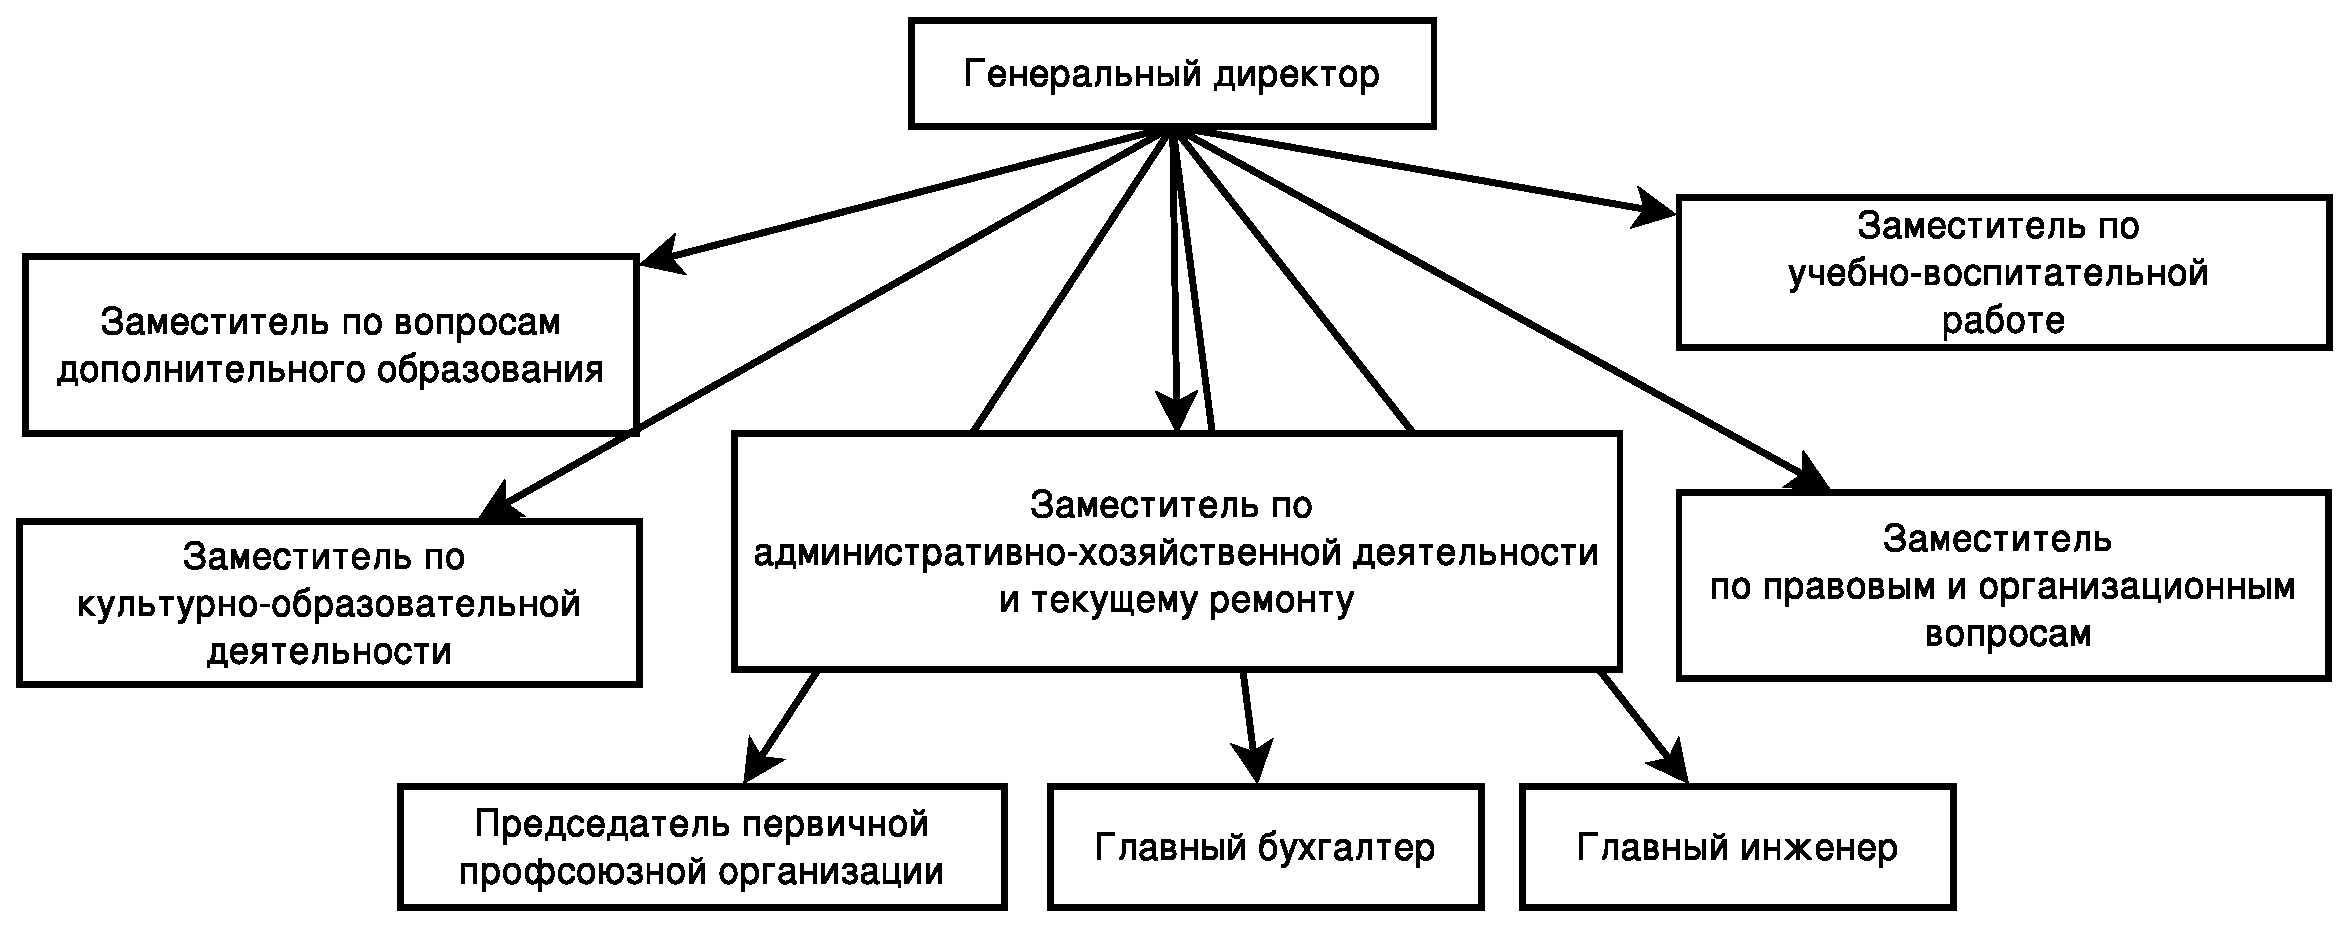
\includegraphics[height=160mm, width=0.8\textwidth, clip, keepaspectratio]{pictures/management_structure.eps}
   \caption{Структура управления организацией}\label{fig:fig_management_struct}
 \end{figure}

Территориальная распределенность обусловленна тем, что Дворец творчества юных расположен в центре города, на его территории находиться множество отдельных корпусов, а также ему принадлежит довольно большой участок земли на Крестовском острове и ЗЦДЮТ <<Зеркальный>>. Доступ пользователей к глобальным и локальным информационным ресурсам обеспечивается подключениями по выделенной линии
(2 мб/с), по оптоволокну (1000 мб/с) и прямыми подключениями к узлу (100 мб/с). Сеть рассчитана на большое количество пользователей ИТ-инфраструктурой (более
15 000 компьютеров). Среди них: работники дворца; педагоги; управляющий персонал;  персонал, отвечающий за сервисную деятельность; учащиеся. Сложность управленческой структуры организации определяется большим штатом сотрудников и широким спектром исполняемых функций. Главным руководителем является генеральный директор, которому подчиняются различные подразделения такие как: финансовый, хозяйственный, учебно-воспитательный и другие сектора.

\begin{figure}[ht]
   \centering%центрируем картинку
   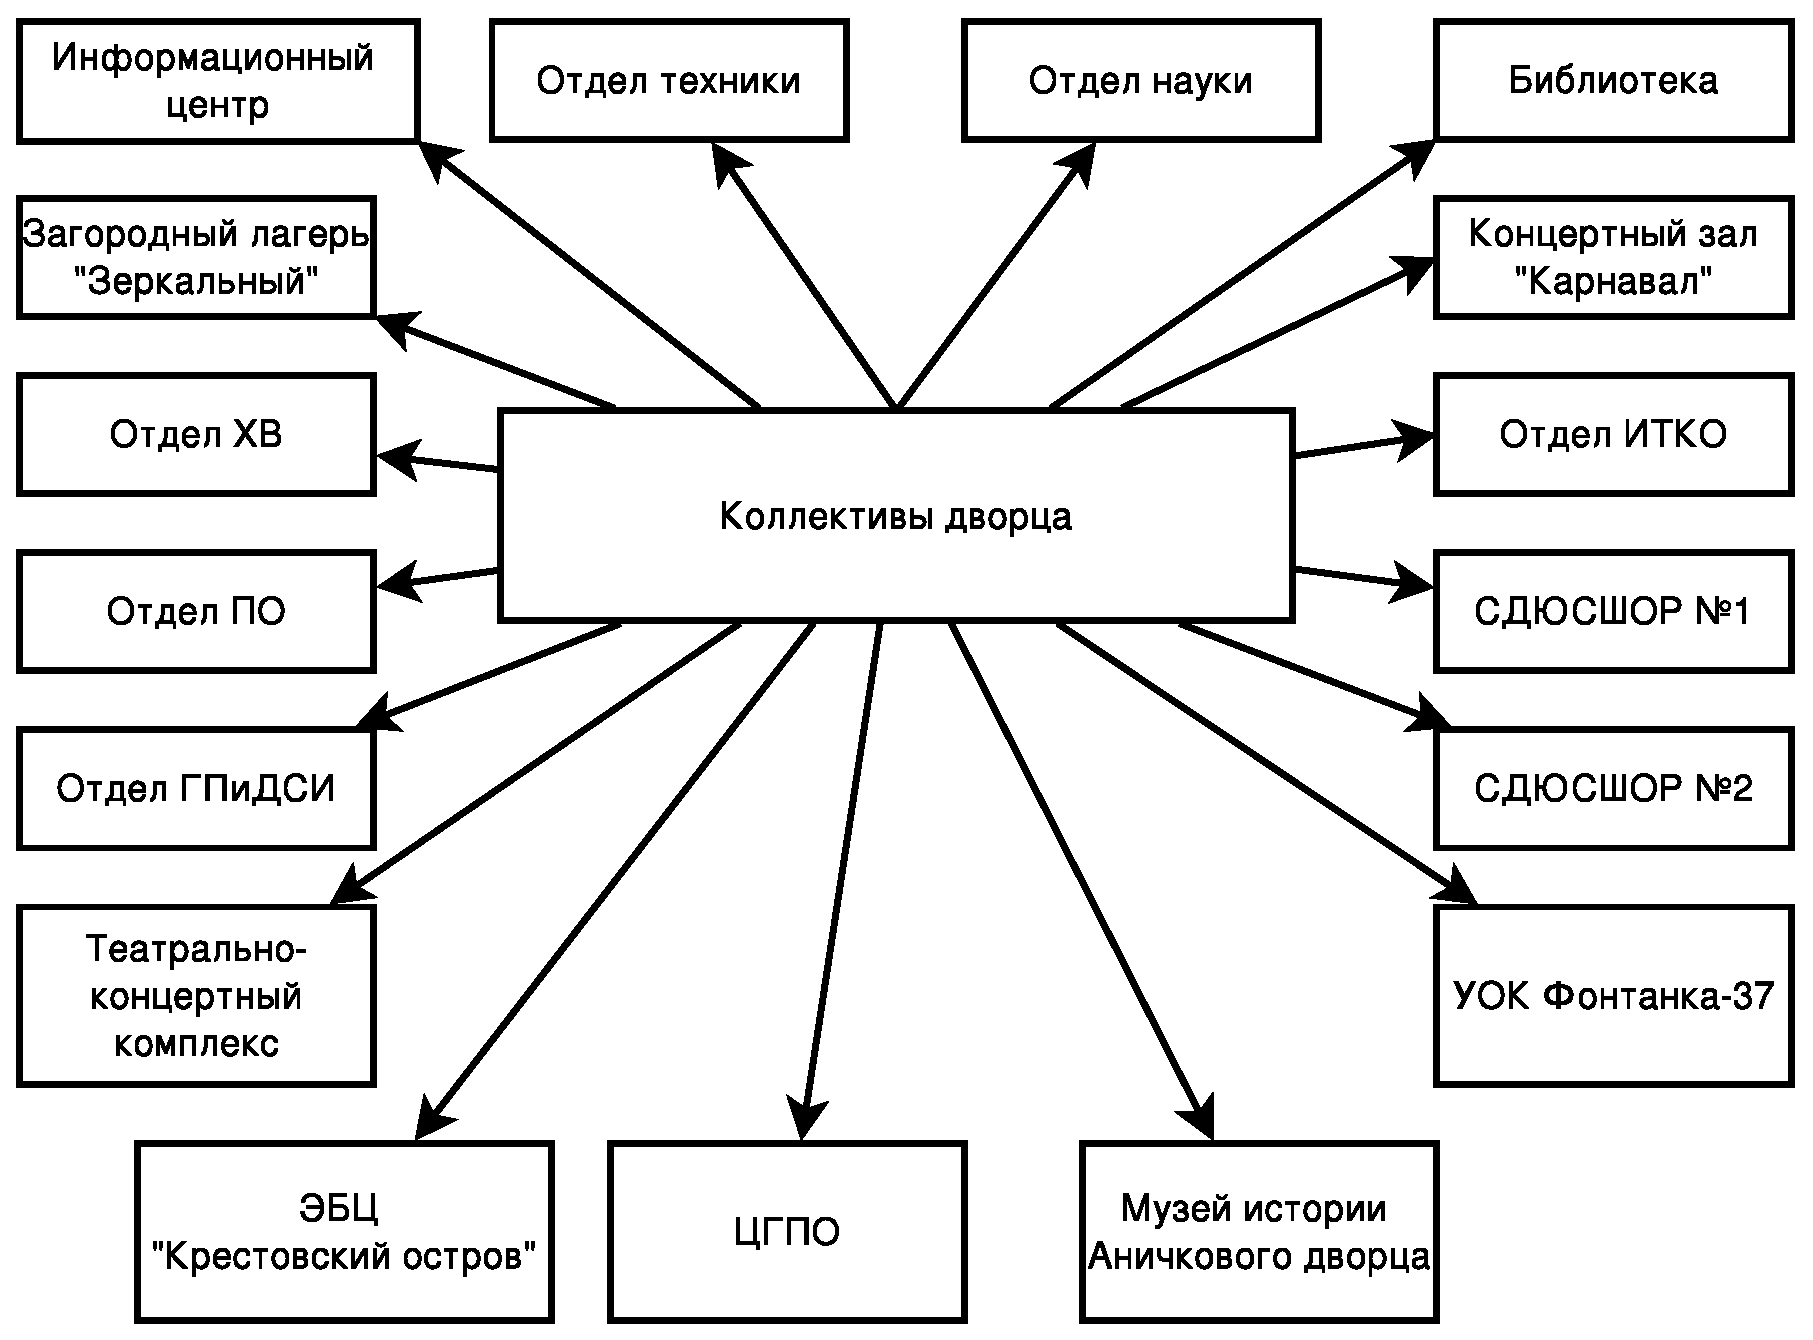
\includegraphics[height=160mm, width=0.8\textwidth, clip, keepaspectratio]{pictures/org_struct.eps}
   \caption{Структура подразделений}\label{fig:org_structure}
 \end{figure}

Сотрудники дворца разделены на коллективы или отделы, отвечающие за определенный вид деятельности(рисунок \ref{fig:org_structure}).
Каждый отдел в свою очередь имеет большое количество своих подразделений. У каждого коллектива или отдела есть свой директор, один или несколько заместителей и большое количество сотрудников.


\begin{itemize}
\item Отдел ХВ – отдел художественного воспитания
\item Отдел ПО – отдел предшкольного  образования
\item Отдел ГПиДСИ – отдел гуманитарных программ и детских социальных инициатив
\item Отдел ИТКО – отдел информационных технологий и компьютерного обеспечения
\item СДЮС школа №1 – специализированная детско-юношеская спортивная школа №1
\item СДЮС школа № – специализированная детско-юношеская спортивная школа №2
\item УОК <<фонтанка-37>> – учебно-оздоровительный комплекс <<фонтанка-37>>
\item ЭБЦ <<крестовский остров>> – эколого-биологический центр <<крестовский остров>>
\item ЦГПО – центр городских предметных олимпиад.
\end{itemize}

Основной функцией дворца является оказание образовательных и воспитательных услуг, которые оказывают учебные коллективы, осуществляющие свою деятельность под управлением методических подразделений самого Дворца
и управляющих организаций МОиН города. Кроме непосредственно обучения сотрудники  составляют различные учебные программы, рабочие планы, отчеты, разрабатывают учебно-методические пособия.
Обеспечением текущей деятельности дворца, в аспекте поддержания в надлежащем состоянии оборудования, коммуникаций занимаются сервисные подразделения Дворца. Схема должностей СПБГТЮ представлена на рисунке \ref{fig:fig_management_struct}.

\subsection{Задачи требующие инфраструктурного сопровождения}\label{ssect:tasks_infra}
Основной функцией дворца является оказание образовательных и воспитательных услуг, предоставление которых оказывают учебные коллективы, осуществляющие свою деятельность под управлением методических подразделений самого Дворца
и управляющих организаций МОиН города. Кроме непосредственно обучения сотрудники составляют различные учебные программы, рабочие планы, отчеты, разрабатывают учебно-методические пособия. 

Для обеспечения работы сотрудников требуется система сетевого хранения файлов по подразделениям с возможностью разделения прав доступа сотрудников. Такое разделение необходимо для того, чтобы . Для разных подразделений это могут быть различные виды файлов: изображения, документы в различных форматах, аудио или видео информация и так далее. Подразделениям необходима возможность выкладывать файлы в общий доступ.

\subsection{Ограничения накладываемые на информационное сопровождение}\label{ssect:restrict_infra}
Поскольку организация осуществляет переход на свободное программное обеспечение, то требуется использование исключительно свободных программных продуктов для реализации системы хрпнения файлов. В проекте используются только компоненты распространяющиеся под свободными лицензиями, одобренными OSI(Open Software Initiative). Решение должно функционировать в операционной системе GNU/Linux и быть независимым от ОС установленной на рабочем месте пользователя.

У педагогов в следствии недостатка времени и иногда отсутствия желания осваивать новый продукт могут возникнуть трудности при переходе на новую информационную систему. С другой стороны, педагоги – люди, которые умеют учиться, что является неоспоримым плюсом для более быстрого перехода на новую систему.

Кроме того, многие педагоги работают не только во Дворце, но и дома, где зачастую используется другое программное обеспечение, в большинстве случаев проприетарное. Следовательно, необходимо предоставить возможность доступа к служебной информации, методическим и др. материалам, необходимым для обеспечения профессиональной деятельности без привязки к определённым операционным системам.

Управленческий аппарат почти весь состоит из людей далёких от информационный технологий. У таких сотрудников нет желания менять устоявшийся бизнес-процесс, поэтому их приходиться заставлять переучиваться, используя административный ресурс, что накладывает жёсткие ограничения на сложность использования системы хранения файлов.

%Сервисные сотрудники обладают большим количеством свободного времени,
%но у них отсутствует желание работать, трудиться, им свойственна лень, поэтому им не хочется учиться, но процесс обучения у них происходит быстрее за счёт имеющихся знаний.

Во Дворце ежедневного находится большое количество сотрудников, выполняющих свои непосредственные обязанности, поэтому функционирование Дворца является непрерывным процессом, поэтому его не только не следует приостанавливать,
а категорически не рекомендуется это делать.

Таким образом система сетевого доступа к файлам должна быть максимально простой с точки зрения пользователя, использовать стандартизованные решения, реализации которых есть под все популярные операционные системы и быть открытым программным обеспечением.

\subsection{Предположительные архитектурные решения и задачи информационной системы}
Исходя из положений раздела~\ref{ssect:tasks_infra} задачей хранилища данных является хранение файлов пользователей, дерева каталогов, информации о пользователях и их правах доступа. В процессе работы, пользователи будут использовать большое количество различных форматов файлов, поэтому представление файла в системе хранения должно быть максимально обобщённым. 

Система ориентирована на пользователей с различным уровнем знакомства с информационными технологиями(раздел~\ref{ssect:restrict_infra}). Для минимизации риска утери данных при случайном удалении или перезаписи файлов требуется реализовать хранение истории версий таким образом, чтобы пользователь мог получить доступ к удалённому файлу или одной из предыдущих доступных версий. В то же время, для уменьшения обьёма данных хранящихся на жестком диске хранилища, требуется возможность окончательного удаления предыдущих версий файлов по прошествии определённого срока администратором системы.

Для осуществления контроля за действиями пользователей и поиска ошибок в работе системы требуется сохранять информацию о действиях пользователей в системе с момента входа в систему. Для поиска проблемы необходимо знать какие действия выполнял пользователь в указанный момент времени и были ли ему разрешены данные действия правами доступа на тот момент.

Таким образом требуется:
\begin{itemize}
\item осуществление разделения пользователей по ролям доступа
\item предоставление удобного доступа пользователя к файлам и директориям, на которые ему были установлены права доступа.
\item хранение предыдущих версий файлов с возможностью их последующего удаления
\item ведение журнала активности пользователей
\end{itemize}

Исходя из требований к системе, предлагается трёхзвенная архитектура: Клиент -- сервер приложений -- хранилище данных. Такая архитектура позволяет разделить логику работы клиент-серверной части и хранения файлов в хранилище данных. 

\section{Обзор аналогов}
\subsection{Samba}

Samba — программа, которая позволяет обращаться к сетевым дискам на различных операционных системах по протоколу SMB/CIFS. 
Имеет клиентскую и серверную части. Является свободным программным обеспечением, выпущена под лицензией GPL. Такая система удобна в использовании, предоставляет удобный доступ клиенту к файлам, не требует предварительной передачи на жёсткий диск пользователя. Минусами данного варианта реализации является ориентированность на работу в локальной сети, отсутствие версионности хранящихся файлов.

\subsection{Системы управления версиями}
Система управления версиями — программное обеспечение для облегчения работы с изменяющейся информацией. Система управления версиями позволяет хранить несколько версий одного и того же документа, при необходимости, возвращаться к более ранним версиям, определять, кто и когда сделал то или иное изменение и многое другое.

Системы контроля версий такие как: git, svn, cvs; требуют определённой подготовки от пользователя. Это решение требует от пользователя ручного получения файлов из хранилища и помещения их обратно. Исходя из причин по которым создавались такие системы, невозможно ограничить глубину сохранения версий файлов, что при использовании не-текстовых данных приводит к быстрому разрастанию хранилища файлов.

Решение на основе git является наиболее безопасным, поскольку все данные передаются через шифрованное соединение, а аутентификация пользователя производится на основе криптографических ключей.

\subsection{Системы электронного документооборота}
Система документооборота, система электронного документооборота (СЭД) — автоматизированная многопользовательская система, сопровождающая процесс управления работой иерархической организации с целью обеспечения выполнения этой организацией своих функций. При этом предполагается, что процесс управления опирается на человеко-читаемые документы, содержащие в слабоформализованной форме инструкции для сотрудников организации, необходимые к исполнению.

Такие системы оориентированы на управление бизнес-процессами и оперируют понятием документа. Организовать в такой системе совместную работу над разнородными материалами, такими как методические пособия сложно, поскольку зачастую это может быть мультимедийная информация к обработке и хранению которой СЭД не приспособлены.

\section{Формализация техического задания}
\subsection{Платформа}
Исходя из ограничений описанных в разделе~\ref{ssect:restrict_infra} требуется использование исключительно свободного ПО для реализации системы хранения файлов. 
\subsection{Средства разработки}

\subsection{Функциональные ограничения}

Требуется ведение журнала активности пользователей, включающего в себя информацию о следующих действиях: 
\begin{itemize}
\item дату и время входа/выхода пользователя
\item создание файла
\item модификация файла
\item удаление файла
\item установка блокировки на файл
\item снятие блокировки с файла
\end{itemize}

Требуется предоставить удобный доступ пользователя к файлам и директориям, на которые ему были установлены права доступа такие как: чтение, запись, удаление файлов и каталогов.

Требуется разработать инструмент позволяющий:	
\begin{itemize}
\item получать информацию об изменениях произошедших с последнего входа пользователя в систему	
\item выполнять аутентификацию пользователя по логину/паролю	
\item выполнять подключение рабочей области пользователя в дерево каталогов
\end{itemize}

Необходимо осуществлять разделение пользователей по следующим ролям:	
\begin{itemize}
\item Пользователь 	в соответствие со своими правами имеет 	доступ к файлам и каталогам подразделения и к общим каталогам. Имеет доступ к предыдущим версиям своих файлов на чтение. 		
\item Администратор подразделения может назначать права 	доступа для сотрудников подразделения, создавать и удалять каталоги в каталоге подразделения. Имеет доступ на чтение к предыдущим версиям файлов подразделения	
\item Администратор создает и удаляет учётные записи пользователей, записи подразделений, назначает права доступа, имеет полный 	доступ к дереву каталогов, имеет полный 	доступ к предыдущим версиям файлов.
\end{itemize}

\chapter{Проектирование}
\section{Системные архитектурные решения}
\subsection{Распределение задач между компонентами}
Бизнес логика реализуется на сервере приложений, в рамках которой обеспечивается:
\begin{itemize}
\item авторизация пользователей, 
\item предоставление требуемых файлов и каталогов для работы в соответствие с правами доступа, 
\item блокировка используемых файлов 
\item получение обновлённой версии с возможным получением предыдущих версий файла.
\item запись информации о действиях пользователей в рамках системы
 \end{itemize}
 
Клиентская часть реализует сетевой доступ к файлам находящимся в хранилище, посредством WebDAV протокола. Задачами клиентской части являются:
\begin{itemize}
\item запрос учётных данных пользователя
\item реализация представления файловой системы и подключение её к дереву каталогов пользователя
\item реализацию протокола общения между клиентской частью и сервером приложений
\item передача файлов пользователя серверу приложений
\item получение запрошенных файлов с сервера приложений
\end{itemize}

Хранилище данных решает задачу хранения пользовательских данных, файлов, дерева каталогов и вспомогательных сущностей.
%\subsection{Описание задач решаемых отдельными компонентами}
\subsection{Описание интерфейсов между компонентами}

\section{Архитектура программы}
\subsection{Архитектура БД}

В проекте используется технология объектно-реляционного отображения, позволяющая работать с записями в БД, как с объектами языка программирования. Такой подход позволяет представить БД как абстрактное хранилище объектов и не задумываться над деталями конкретной реализации БД.

Для хранения данных может использоваться любая реляционная СУБД, которая поддерживается выбранной библиотекой для объектно-реляционного отображения.

\begin{figure}[ht]
   \centering%центрируем картинку
   \includegraphics[height=160mm, width=0.8\textwidth, clip, keepaspectratio]{pictures/DB.eps}
   \caption{Схема БД}\label{fig:db_scheme}
 \end{figure}

Основные сущности используемые в системе показаны на рисунке \ref{fig:db_scheme}. В БД хранится информация о пользователях, группах, правах доступа, хранящихся файлах их содержимом и версиях.
 
\subsection{Архитектура клиентской части}

Клиентская часть реализует доступ к файловому хранилищу как к подкаталогу в дереве файлов пользователя. Это достигается использованием средств, которые позволяют предоставить POSIX интерфейс к сетевому хранилищу данных.

\begin{figure}[ht]
   \centering%центрируем картинку
   \includegraphics[height=160mm, width=0.8\textwidth, clip, keepaspectratio]{pictures/client_sequencs.eps}
   \caption{Схема взаимодействия клиента с сервером приложений}\label{fig:client_sequence}
 \end{figure}

На диаграмме последовательностей (рисунок \ref{fig:client_sequence}) показаны события происходящие в процессе работы пользователя с файловой системой. В работе пользователя выделяются три основных этапа: монтирование, изменение объектов файловой системы и отмонтирование системы. 

При монтировании ФС, у пользователя запрашивают его логин/пароль для работы в системе, после этого сервер приложений проверяет правильность введённых данных и аутентифицирует его и возвращает содержимое корневой директории пользователя.

При изменениии файла происходит блокировка ресурса на сервере приложений. Запись данных пользователем идёт в локальный кэш, который через некоторое время отправляется на сервер приложений. Использование кеширования позволяет уменьшить количество версий файлов, особенно для приложений в которых используется автосохранение файлов.

При отмонтировании происходит оттравка данных из кеша клиентской части на сервер приложений и отключение от сервера приложений.

\subsection{Архитектура сервера приложений}

Сервер приложений используется для обработки запросов пользователей и подготовкой полученных файлов к сохранению в хранилище. Сервер приложений состоит из многопоточного обработчика запросов пользователей, обработчика аутентификации и авторизации пользователей и обработчика davfs протокола используемого для связи с клиентским приложением.

\begin{figure}[ht]
   \centering%центрируем картинку
   \includegraphics[height=160mm, width=0.8\textwidth, clip, keepaspectratio]{pictures/davstorage.eps}
   \caption{Диаграмма значимых классов проекта}\label{fig:davstorage}
 \end{figure}
 
 Диаграмма классов системы, без реализации WebDAV и http-сервера представлена на рисунке \ref{fig:davstorage}. Система постоена на принципе независимости от реализации хранения файлов и информации о пользователях, что позволяет реализовать своё хранилище данных, реализующее интерфейс для WebDAV протокола.

\section{Проектирование инфраструктуры}
\subsection{Оценка требований к серверу}
\subsection{Оценка требований к рабочему месту пользователя}
\subsection{Оценка требований к пропускной способности канала}

\chapter{Реализация}
\section{Особенности реализации БД}
В проекте используется технология объектно-реляционного отображения, позволяющая работать с записями в БД, как с объектами языка программирования. Такой подход позволяет представить БД как абстрактное хранилище объектов и не задумываться над деталями конкретной реализации БД. 

\section{Особенности реализации инструмента администрирования}

\section{Особенности реализации клиентской части}
Клиентская часть состоит из модуля к FUSE, утилит монтирования и графического интерфейса для утилит монтирования для упрощения работы пользователям. 

\begin{figure}[ht]
   \centering%центрируем картинку
   \includegraphics[height=160mm, width=0.8\textwidth, clip, keepaspectratio]{pictures/fuse_structure.eps}
   \caption{Схема работы FUSE}\label{fig:fuse_structure}
 \end{figure}

Filesystem in Userspace (FUSE) (Файловая система в пользовательском пространстве)~—~это модуль для ядер Unix-подобных ОС, с открытым исходным кодом и относящийся к свободному программному обеспечению. Модуль распространяется под лицензиями GNU GPL и GNU LGPL. Он позволяет пользователям без привилегий создавать их собственные файловые системы без необходимости переписывать код ядра. Это достигается за счёт запуска кода файловой системы в пространстве пользователя, в то время как модуль FUSE только предоставляет «мост» для актуальных интерфейсов ядра. Общий принцип работы показан на рисунке~\ref{fig:fuse_structure}. FUSE особенно полезна для написания виртуальных файловых систем. В отличие от традиционных файловых систем, которые по существу сохраняют информацию для восстановления данных с диска, виртуальные файловые системы не хранят данные непосредственно. Они действуют как представление, трансляция (перевод) существующей файловой системы или устройства хранения. Практически, любой ресурс, доступный для использования FUSE, может быть экспортирован в файловую систему.

Для реализации управления версионированием для проекта davfs2 была реализована возможность задания расширеных атрибутов файловой системы. 

Расширенные атрибуты файловой системы - это ассоциированый с элементом ФС набор метаданных не связанных с файловой системой. Такой набор метаданных реализован в виде ассоциативного массива хранящего имя атрибута и его значения в виде текстовых строк. В ОС GNU/Linux имя атрибута является строкой заканчивающейся нулевым символом и должно предваряться пространством имён. Используется пространство имен "user" поскольку список атрибутов которые могут в нём содержаться не ограничен. Эта возможность используется для управления версионностью файлов хранящихся в директории. При установке атрибута "user.history" для директории, создаётся подкаталог ".history" в котором содержатся записи истории изменения файлов.



\section{Особенности тестирования и отладки}
\section{План внедрения и отладки}
\subsection{Организационные мероприятия}
\subsection{Технические мероприятия}
\subsection{Мероприятия сопровождения}

\chapter{Экономическая часть}
\chapter{Безопасность жизнедеятельности при разработке информационной системы}
Целью является обоснование мер безопасности и анализ опасных, вредных производственных факторов воздействия на оператора ПЭВМ.
Общая же система мероприятий по безопасности труда должна соответствовать требованиям СанПиН 2.2.2/2.4.1340-03 <<Гигиенические требования к персональным электронно-вычислительным машинам и организации работы>>. 

\section{Анализ опасных и вредных производственных факторов при работе с компьютером}
\label{safety_analysis}
В соответствие с ГОСТ 12.0.003 – 03 <<Классификация опасных и вредных производственных факторов>> (ОВПФ). ОВПФ подразделяются на следующие группы по природе действия: физические, химические, биологические и психофизиологические.

\subsection{Физические ОВПФ}
Повышенная или пониженная температура воздуха рабочей зоны, повышенная или пониженная влажность воздуха рабочей зоны. Могут вызывать дискомфорт, снизить работоспособность, повысить утомляемость работающих.
Повышенная или пониженная ионизация воздуха. Электрооборудование влияет на уровень ионизации воздуха в процессе работы, что приводит к ухудшению здоровья, расстройству нервной системы, гипоксии.
Повышенный уровень шума, вибрации на рабочем месте.  Шум негативно влияет на нервную и сердечнососудистую системы, а также на органы пищеварения.
Повышенный уровень ультрафиолетовой радиации, повышенный уровень инфракрасной радиации. Источником ИК и УФ излучения является монитор. Воздействие УФ излучения сказывается при длительной работе с компьютером или при заболевании сетчатки глаза. Однако, в настоящее время уровни УФ излучения компьютера много ниже допустимого уровня и практически не влияют на состояние здоровья оператора.
Недостаточная освещенность рабочей зоны. Недостаточная освещенность приводит к значительному снижению производительности, приводит к возникновению профессионального заболевания – близорукости.
Повышенное значение напряжения в электрической цепи, замыкание которой может произойти через тело человека. 

\subsection{Химические ОВПФ}
Содержание вредных веществ в производственных помещениях не должно превышать значений предельно допустимых концентраций (ПДК) вредных веществ в воздухе населенных мест (ГОСТ 12.1.005-88 ССБТ. <<Общие санитарно–гигиенические требования к воздуху рабочей зоны>>).

\subsection{Биологические ОВПФ}
Биологические ОВПФ включают в себя микро и макроорганизмы, влияющие на здоровье человека. При существенном их количестве в несколько раз увеличивается риск заболеваний. Патогенные микроорганизмы (вирусы, грибки, бактерии) и макроорганизмы (растения, животные) при регулярной и качественной уборке помещения не скапливаются.

\subsection{Психофизиологические ОВПФ}
Умственное перенапряжение. Вызывает ухудшение памяти, плохой сон, головные боли и др.
Повышенные нервно-эмоциональные перегрузки.
Монотонность труда. Следствие: труднее переключиться на другую работу (требуется небольшой отдых).
Перенапряжение зрительных и слуховых анализаторов.
Длительные статические нагрузки. Вызывает усталость мышц спины, шеи, рук и ног.
Неправильная организация рабочего места и порядка работы может приводить к заболеваниям нервной системы, таким как: стресс, стенокардия и головные боли; заболеваниям костно-мышечной системы: ревматизм, остеохондроз, радикулит, запястный синдром и синдром длительных статических нагрузок (СДСН); заболеваниям глаз: близорукость, воспалительные заболевания глаз, катаракта, отслоение сетчатки, косоглазие.
Воздействие указанных неблагоприятных факторов приводит к снижению работоспособности, вызванное развивающимся утомлением. Появление и развитие утомления связано с изменениями, возникающими во время работы в центральной нервной системе, с тормозными процессами в коре головного мозга.

\section{Обеспечение безопасности работ на рабочем месте}
Вследствие анализа опасных и вредных производственных факторов представленного в разделе~\ref{safety_analysis}, следует предложить следующие меры безопасности при работе пользователей с ПЭВМ.

\subsection{Обеспечение электробезопасности}
С целью предупреждения поражений электрическим током, в соответствии с правилами электробезопасности, в служебном помещении должен осуществляться постоянный контроль состояния электропроводки, предохранительных щитов, шнуров, с помощью которых включаются в электросеть компьютеры, осветительные приборы, другие электроприборы. 
Исключительно важное значение для предотвращения электротравмотизма имеет правильная организация обслуживания действующих электроустановок ИО, проведения ремонтных, монтажных и профилактических работ согласно ГОСТ 12.1.030-81. ССБТ. <<Электробезопасность. Защитное заземление, зануление>>.
В ИО разрядные токи статического электричества чаще всего возникают при прикосновении к любому из элементов ЭВМ. Такие разряды опасности для человека не представляют, но кроме неприятных ощущений они могут привести к выходу из строя ЭВМ. Для снижения величины возникающих зарядов статического электричества в ИО покрытие технологических полов следует выполнять из однослойного поливинилхлоридного антистатического линолеума. В помещении должна отсутствовать электрически активная среда, отсутствовать возможность одновременного прикосновения к металлическим частям прибора и заземляющему устройству, отсутствовать высокая температура и сырость (ПТЭЭП 6 от 13.01.2003г.). Другим методом защиты является нейтрализация заряда статического электричества ионизированным газом. К общим мерам защиты от статического электричества в ИО можно отнести общие и местное увлажнение воздуха. 

\subsection{Обеспечение санитарно-гигиенических требований к помещениям ИО и рабочим местам операторов ПЭВМ}
Помещения ИО, их размеры (площадь, объем) должны в первую очередь соответствовать количеству работающих и размещаемому в них комплекту технических средств. В них предусматриваются соответствующие параметры температуры, освещения, чистоты воздуха, обеспечивают изоляцию, от производственных шумов и т.п. Для обеспечения нормальных условий труда санитарные нормы СН 245-71 устанавливают 
на одного работающего, объем производственного помещения не менее 15 м\textsuperscript{3}, площадь помещения выгороженного стенами или глухими перегородками не менее 4,5 м\textsuperscript{3}. 

\subsection{Требования к освещенности рабочей зоны}
В ИО, как правило, применяется боковое естественное освещение. Рабочие комнаты и кабинеты должны иметь естественное освещение, коэффициент естественной освещенности обязан быть не менее 1,2-1,5\%, согласно СанПиН 2.2.2/2.4.1340-03. В тех случаях, когда одного естественного освещения не хватает, устанавливается совмещенное освещение.

Искусственное освещение по характеру выполняемых задач делится на рабочее, аварийное, эвакуационное. 
Искусственное освещение помещений и рабочих мест с ПЭВМ должно осуществляться системой общего равномерного освещения. 
Освещенность на поверхности стола в зоне размещения рабочего документа должна быть 300-500 лк (СанПиН 2.2.2/2.4.1340-03). Для обеспечения такого уровня освещенности допускается установка светильников местного освещения для подсветки документов. В тоже время местное освещение не должно увеличивать освещенность экрана более 300 лк и создавать бликов на поверхности экрана. 
Рациональное цветовое оформление помещения направленно на улучшение санитарно-гигиенических условий труда, повышение его производительности и безопасности. Окраска помещений ИО влияет на нервную систему человека, его настроение и, в конечном счете, на производительность труда. Основные производственные помещения целесообразно окрашивать в соответствии с цветом технических средств. Освещение помещения и оборудования должно быть мягким, без блеска. 
Показатель ослепленности для источников общего искусственного освещения в производственных помещениях должен быть не более 20. Коэффициент запаса для осветительных установок общего освещения должен приниматься равным 1,4. Следует ограничивать прямую блесткость от источников освещения. При этом яркость светящихся поверхностей, находящихся в поле зрения, должна быть не более 200 кд/м\textsuperscript{2}. 
Следует ограничивать отраженную блескость на рабочих поверхностях за счет правильного выбора типов светильников и расположения рабочих мест по отношению к источникам естественного и искусственного освещения, при этом яркость бликов 
на экране ПЭВМ не должна превышать 40 кд/м\textsuperscript{2} и яркость потока, при изменении системы отраженного освещения, не должна превышать 200 кд/м\textsuperscript{2}.
Дизайн ПЭВМ должен предусматривать окраску корпуса в спокойные мягкие тона с диффузным рассеиванием света. Корпус ПЭВМ, клавиатура и другие блоки и устройства ПЭВМ должны иметь матовую поверхность одного цвета с коэффициентом отражения 0.4 - 0.6 и не иметь блестящих деталей, способных создавать блики.

\subsection{Требования к организации рабочего места пользователя}
По СанПиН 2.2.2/2.4.1340-03 при конструировании оборудования и организации рабочего места пользователя ПЭВМ следует обеспечивать соответствие конструкции всех элементов рабочего места и их взаимного расположения эргономическими требованиями с учетом характера выполняемой пользователем деятельности, комплексности технических средств, форм организации труда и основного рабочего положения пользователя.
В качестве основных эргономических требований организации рабочего места пользователя выбираются следующие:
\begin{itemize}
 \item особенности конструктивного выполнения и расположения технических средств и аппаратуры;
 \item длительность работы с данной аппаратурой;
 \item точность и эффективность приема информации.
\end{itemize}

Первый принцип определяется выбранной аппаратурой, тогда как второй и третий зависят от первого и определяют функциональное состояние пользователя.
Экран видеомонитора должен находиться от глаз пользователя на расстоянии 600-700 мм, но не ближе 500 мм с учетом размеров алфавитно-цифровых знаков и символов.
Положение тела должно соответствовать направлению взгляда. Расположение клавиатуры не должно приводить к напряжению рук.
Для ввода данных из документов (бланков), их рекомендуется располагать 
на расстоянии 450-500 мм от глаз пользователя, преимущественно слева, при этом угол между экраном монитора и документом в горизонтальной плоскости не должен превышать 30-40 градусов.
Время непрерывной работы – 45 минут. Перерыв – 15 минут. В перерыве – физические упражнения с растяжением мышц спины и рук. Суммарное рабочее время за сутки 4 часа.

Высота рабочей поверхности стола для пользователей должна регулироваться в пределах 680-800 мм; при отсутствии таковой возможности высота рабочей поверхности стола должна составлять 725 мм.Рабочий стол должен иметь пространство для ног высотой не менее 600 мм, шириной – не менее 500 мм, глубиной на уровне колен – не менее 450 мм и на уровне вытянутых ног – не менее 650 мм. Рабочий стул (кресло) должен быть подъемно-поворотным и регулируемым по высоте и углам наклона сиденья и спинки, а также – расстоянию спинки до переднего края сиденья.
Рабочее место пользователя ПЭВМ следует оборудовать подставкой для ног, имеющей ширину не менее 300 мм, глубину не менее 400 мм, регулировку по высоте в пределах до 150 мм и по углу наклона опорной поверхности подставки до 20 . Поверхность подставки должна быть рифленой и иметь по переднему краю бортик высотой 10 мм.
Клавиатуру следует располагать на поверхности стола на расстоянии 100-300 мм от края, обращенного к пользователю, или на специальной регулируемой по высоте рабочей поверхности, отделенной от основной столешницы.

\subsection{Меры по снижению уровня шума}
Снижение шума, создаваемого на рабочих местах ИО внутренними источниками, а также шума проникающего извне, является очень важной задачей. В соответствии с ГОСТ 12.1.003-83 <<ССБТ. Шум. Общие требования безопасности>>, снижение шума в источнике излучения можно обеспечить применением упругих прокладок между основанием машины, прибора и опорной поверхностью. В качестве прокладок используются резина, войлок, пробка, различной конструкции амортизаторы. Под настольные шумящие аппараты можно подкладывать мягкие коврики из синтетических материалов, а под ножки столов, на которых они установлены, – прокладки из мягкой резины, войлока, толщиной 6-8 мм. Крепление прокладок возможно путем приклейки их к опорным частям. 
Снижение уровня шума, проникающего в производственное помещение, может быть достигнуто увеличением звукоизоляции ограждающих конструкций, уплотнением по периметру притворов окон, дверей. 
Таким образом, для снижения шума создаваемого на рабочих местах внутренними источниками, а также шума проникающего извне следует:
\begin{itemize}
 \item ослабить шум самих источников (применение экранов, звукоизолирующих кожухов);
 \item снизить эффект суммарного воздействия отраженных звуковых волн (звукопоглощающие поверхности конструкций);
 \item применять рациональное расположение оборудования;
 \item использовать архитектурно-планировочные и технологические решения изоляций источников шума.
\end{itemize}

\section{Пожарная безопасность}
Основы обеспечения пожарной безопасности определены Федеральным законом №69 <<О пожарной безопасности>> от 21.12.1994 г. Основы противопожарной защиты предприятий определены стандартами: ГОСТ 12.1.004-91 <<Пожарная безопасность. Общие требования>> и ГОСТ 12.1.010-76 <<Взрывобезопасность. Общие требования>>.
Пожарная безопасность обеспечивается системой предотвращения пожара и системой пожарной защиты. Во всех служебных помещениях обязательно должен быть <<План эвакуации людей при пожаре>>, регламентирующий действия персонала в случае возникновения очага возгорания и указывающий места расположения пожарной техники. 
Пожары в ИО представляют особую опасность, так как сопряжены с большими материальными потерями. Характерная особенность ИО – небольшие площади помещений. 
Источниками зажигания в ИО могут быть электронные схемы от ЭВМ, приборы, применяемые для технического обслуживания, устройства электропитания, кондиционирования воздуха, где в результате различных нарушений образуются перегретые элементы, электрические искры и дуги, способные вызвать загорания горючих материалов. 
Для большинства помещений ИО установлена категория пожарной опасности <<В>>. 
Учитывая высокую стоимость электронного оборудования ИО, а также категорию его пожарной опасности, здания для ИО и части здания другого назначения, в которых предусмотрено размещение ЭВМ должны быть 1 и 2 степени огнестойкости. 
В зданиях ИО пожарные краны устанавливаются в коридорах, на площадках лестничных клеток и входов. Применение воды в машинных залах ЭВМ, хранилищах носителей информации, помещениях контрольно-измерительных приборов ввиду опасности повреждения или полного выхода из строя дорогостоящего оборудования возможно в исключительных случаях, когда пожар принимает угрожающе крупные размеры. При этом количество воды должно быть минимальным, а устройства ЭВМ необходимо защитить от попадания воды, накрывая их брезентом или полотном. 
Для тушения пожаров на начальных стадиях широко применяются огнетушители. По виду используемого огнетушащего вещества огнетушители подразделяются 
на следующие основные группы. 
Пенные огнетушители, применяются для тушения горящих жидкостей, различных материалов, конструктивных элементов и оборудования, кроме электрооборудования, находящегося под напряжением.
Газовые огнетушители применяются для тушения жидких и твердых веществ, а также электроустановок, находящихся под напряжением. 
В производственных помещениях ИО применяются главным образом углекислотные огнетушители, достоинством которых является высокая эффективность тушения пожара, сохранность электронного оборудования, диэлектрические свойства углекислого газа, что позволяет использовать эти огнетушители даже в том случае, когда не удается обесточить электроустановку сразу. 
Объекты ИО необходимо оборудовать установками стационарного автоматического пожаротушения. Наиболее целесообразно применять в ИО установки газового тушения пожара, действие которых основано на быстром заполнении помещения огнетушащим газовым веществом с резким сжижением содержания в воздухе кислорода.
Меры пожарной безопасности определены по НПБ 110-03. Пользователи допускаются к работе на персональных ЭВМ только после прохождения инструктажа по безопасности труда и пожарной безопасности на каждом рабочем месте.
Профилактические методы борьбы с пожарами на рабочем месте оператора ПЭВМ предусматривают:
организационные: правильное содержание помещений, противопожарный инструктаж служащих, издание приказов по вопросам усиления пожарной безопасности 
и т.д.;
технические: соблюдение противопожарных правил, норм при проектировании помещений, при устройстве электропроводов и оборудования, отопления, вентиляции, освещения;
режимные: запрещение курения в не установленных местах, производство пожароопасных работ в помещении машинного зала и т.д.;
эксплуатационные: своевременные профилактические осмотры, ремонты оборудования.
Необходимо предусмотреть безопасную эвакуацию людей на случай возникновения пожара. В соответствии с НПБ 104-03 число эвакуационных выходов из зданий, помещений должно составлять не менее двух.

\section{Заключение}
Проанализированы вредные и опасные для здоровья человека факторы при работе в качестве оператора ЭВМ. Также сделан анализ факторов, не связанных с работой вычислительной техники, но определяющий безопасность работы. Были приведены требования к организации рабочего места. Рабочее место оператора ЭВМ должно быть наиболее комфортабельным и способствовать высокой эффективности труда оператора.


\section{Источники}
\begin{enumerate}
\item Федеральный закон №69 <<О пожарной безопасности>> от 21.12.1994 г.
\item СанПиН 2.2.2/2.4.1340-03 <<Гигиенические требования к персональным электронно-вычислительным машинам и организации работы>>.
\item ГОСТ 12.0.003-03 <<Классификация опасных и вредных производственных факторов>>.
\item ГОСТ 12.1.005-88 ССБТ. <<Общие санитарно–гигиенические требования к воздуху рабочей зоны>>.
\item ГОСТ 12.1.030-81 ССБТ. <<Электробезопасность. Защитное заземление, зануление>>.
\item ГОСТ 12.2.032-78 ССБТ. <<Рабочее место при выполнении работ сидя. Общие эргономические требования>>.
\item ГОСТ 12.1.003-83 ССБТ. <<Шум. Общие требования безопасности>>.
\item ГОСТ 12.1.010-76 <<Взрывобезопасность. Общие требования>>.
\item ГОСТ 12.1.004-91 <<Пожарная безопасность. Общие требования>>.
\end{enumerate}

\Conclusion
заключение

\end{document}